\section{Original Description}

The overarching goal of this project is to design and construct a prototype of an alien surveillance system for OSNAP.  The surveillance system will analyze separately collected video on various server architectures to take advantage of larger core counts and advanced architecture features. The matrix computations associated with Kalman Filters and independent nature of tracking separate objects present excellent possibilities for parallelism.

 The matrix calculations used in the computation of the Kalman Filters can make use of Intel's vector instructions to exploit small-scale data parallelism. This processes will be completed using the vector operations associated with Cilk. Similarly, thread level parallelism can be exploited in the area of tracking. Each tracked object requires a separate Kalman Filter operating on almost entirely independent data which should allow for significant performance improvement through thread level parallelism. TBB will be used to implement this improvement.

\begin{figure}
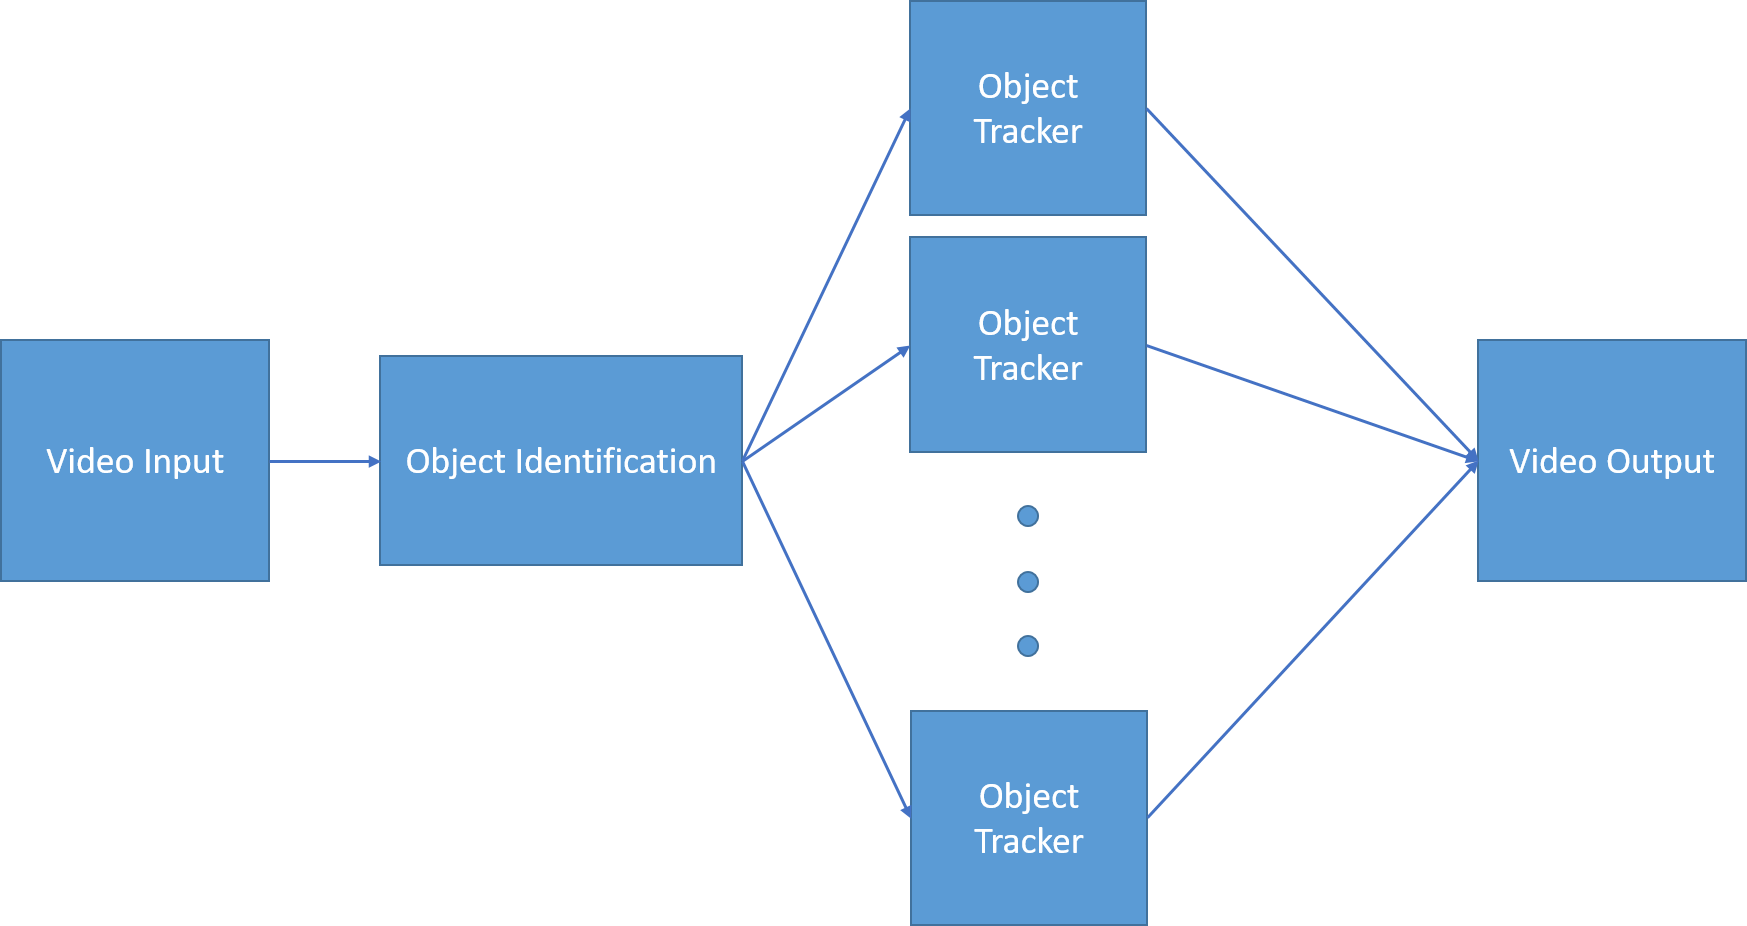
\includegraphics[width=\textwidth]{./arch.png}
\label{fig}
  \caption{General system architecture}
\end{figure}


In figure 1 of the system architecture, it is obvious that the main area of interest for this project is the design and implementation of the object tracking portion of the system since it is in parallel. Although sources of parallelism exist in other aspects of the system those will be left for future work. The object tracking section can be parallelized by treating individual objects separately and by utilizing vector architectures to parallelize the underlying calculations.